\documentclass[11pt]{report}

\usepackage[dutch]{babel}
\usepackage{latexsym}
\usepackage{amssymb}
\usepackage{amsmath}
\usepackage{wasysym}
\usepackage{bm}
\usepackage{graphicx}

\begin{document}
\subsection*{Ratio-meetniveau voor het Rasch model.}
Om na te gaan of een bewering geldt onder het ratio-meetniveau dienen we na te gaan of een trekscore $\theta_{v}$ tot op een constante $q$ kan worden geschreven zonder verlies van betekenis (cfr. Zinvolle vs. zinloze beweringen in de curus \textit{Statistiek I}). Hiervoor dienen we in de formulering na te gaan of, indien we $\theta_{v}'=q\theta_{v}$ gebruiken, we opnieuw bij een gelijke formulering zoals de oorspronkelijke $\theta_{v}$ kunnen komen.

We vertrekken van $\theta_{v}'=q\theta_{v}$. Aangezien de trekscore ($\theta_{v}$) op een factor na (basisveronderstelling voor metingen tot op het ratio-meetniveau)  bepaald is moet er ook bij de $b_{i}$ een aanpassing worden gedaan. Deze moet namelijk ook tot op een factor na gedefini\"eerd worden, aangezien $b_{i}$ in rechtstreeks verband staat met de latente trekscore $\theta(')$. Dus $b_{i}'=qb_{i}$. Naast deze twee aanpassingen dient ook $a$ aangepast te worden indien we wensen na te gaan of een meting tot op ratio-meetniveau bepaald is. Dit is omdat $P(i| \theta_{v}=0) = p_{0}$ op een ratio-schaal gelijk blijft ongeacht de waarde van $q$, als gevolg moet  $P(i| \theta'_{v}=0) = P(i| q\theta_{v}=0) = p_{0}$. Bovendien is $P(i| \theta'_{v}=qb_{i}) = P(i| \theta_{v}=b_{i}) = 1/2$ (grijze lijn). Als gevolg hiervan liggen twee punten op de curve $\Psi$ vast. Dit leidt tot een aanpassing van $a$ tot $a'=a/q$. Zie Figuur 1.

\begin{figure}[h]
\begin{center}
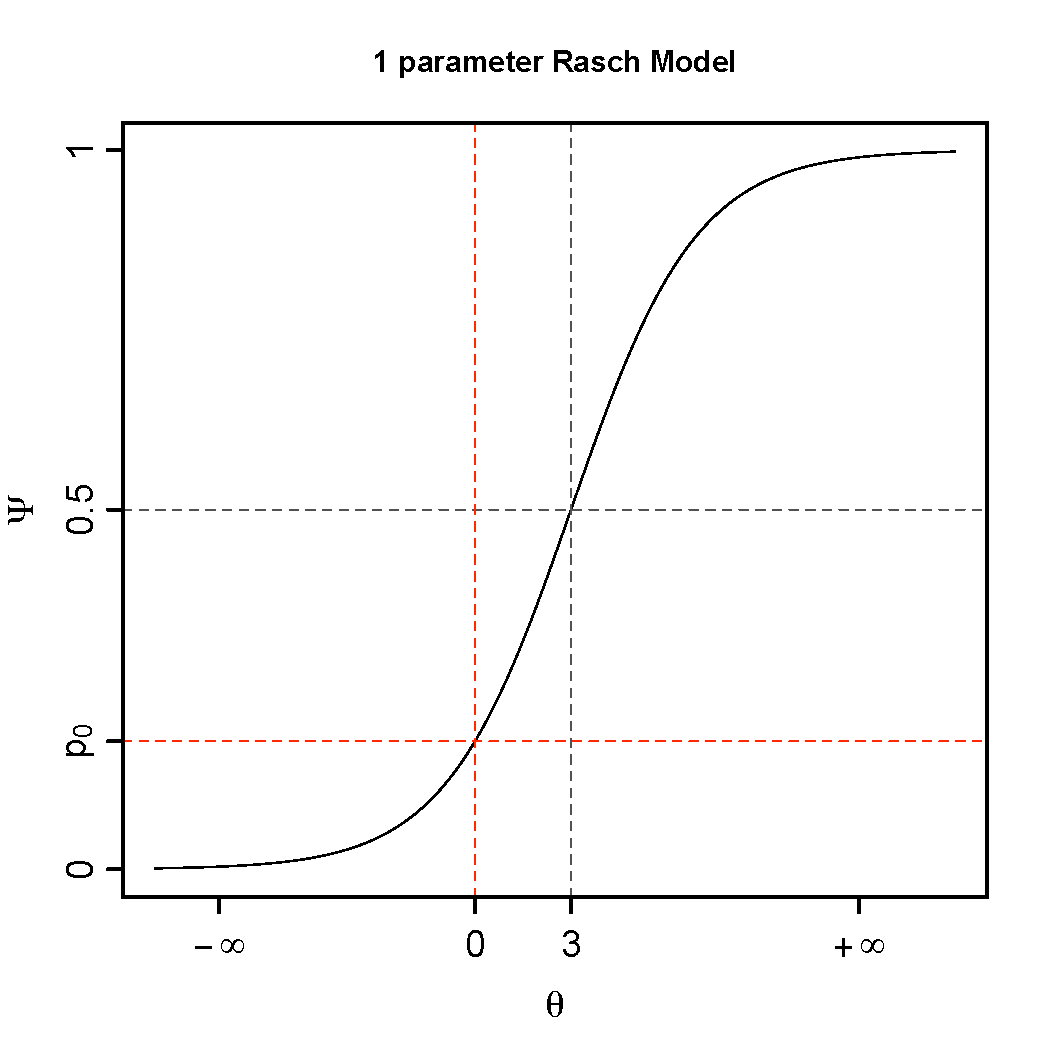
\includegraphics[width=0.5\textwidth]{addi-multi.pdf}
\caption{Een parameter Rasch model met aanduiding van de punten $(\theta(')_{v}=0, p_{0})$ en $(\theta(')_{v}=b(')_{i}, 0.5)$ }
\label{default}
\end{center}
\end{figure}


Bijgevolg hebben we als beginstap in het oplossen (1). Via de uitwerking in (2) en de herschikking in (3) zien we dat de gevraagde gelijkheid in (1) opgaat.

\begin{eqnarray}
\Psi \{1.7[a(\theta_{v}-b_{i})] \} &?=?& \Psi \{1.7[a'(\theta'_{v}-b'_{i}) \}\\
\nonumber \\
\Psi \{1.7[a'(\theta'_{v}-b'_{i})] \} &=& \dfrac{e^{1.7a/q(q\theta_{v}-qb_{i})}}{1+e^{1.7a/q(q\theta_{v}-qb_{i}})}\\
&=& \dfrac{e^{1.7a/q(q)(\theta_{v}-b_{i})}}{1+e^{1.7a/q(q)(\theta_{v}-b_{i})}} \\
&=& \dfrac{e^{1.7a(\theta_{v}-b_{i})}}{1+e^{1.7a(\theta_{v}-b_{i})}}
\end{eqnarray}

\subsection*{Additieve en Multiplicatieve constante}
\subsubsection*{Additieve constante}
Met betrekking tot de multiplicatieve en additieve factor die vermeld worden gelden volgende zaken. In de additieve formulering zoals op slide 13 wordt vermeld dat de parameters $\xi_{v}$ en $\sigma_{i}$ zijn waarvoor geldt:
\begin{itemize}
\item $\mathbf{\bm\xi_{v}=1.7a\bm\theta_{v}}$ subject ability
\item $\mathbf{\bm\sigma_{i}=1.7b_{i}}$ itemmoelijkheid
\end{itemize}

Indien er staat dat de parameters tot op een additieve constante bepaald zijn bedoelt men dat zowel $\xi_{v}$ als $\sigma_{i}$ kunnen herschreven worden als $\xi'_{v} = 
\xi_{v} + s$ en $\sigma'_{i} = \sigma_{i}+s$. Dit is eenvoudig na te gaan. Via de definitie in (5) komt men tot het gevraagde: ``Is het inderdaad zo dat het opgaat voor een additieve constante?'' (Vandaar de notering met de vraagtekens.). De uitwerking van (7) leidt tot de oplossing van het gevraagde. Hierdoor is het bewezen dat in de additieve formulering de parameters $\xi_{v}$ en $\sigma_{i}$ tot op een additieve constante $s$ bepaald zijn.
\begin{eqnarray}
\Psi \{1.7[a(\theta_{v}-b_{i})] \} &=& \dfrac{e^{\xi_{v}-\sigma_{i}}}{1+e^{\xi_{v}-\sigma_{i}}}\\
&?=?& \dfrac{e^{\xi'_{v}-\sigma'_{i}}}{1+e^{\xi'_{v}-\sigma'_{i}}}\\
\nonumber\\
\dfrac{e^{\xi'_{v}-\sigma'_{i}}}{1+e^{\xi'_{v}-\sigma'_{i}}} &=& \dfrac{e^{\xi_{v}+s-(\sigma_{i}+s)}}{1+e^{\xi_{v}+s-(\sigma_{i}+s)}}\\
&=& \dots \nonumber
\end{eqnarray}

\subsubsection*{Multiplicatieve constante}
Indien we dezelfde notatie gebruiken voor de multiplicatieve schrijfwijze als in de additieve schrijfwijze komen we tot volgende defini\"ering van de parameters $\epsilon_{i}$ en $\lambda_{v}$:
\begin{itemize}
\item $\mathbf{\bm\lambda_{v}=e^{\bm\xi_{v}}}$ subject ability
\item $\mathbf{\bm\epsilon_{i}=e^{-\bm\sigma_{i}}}$ item\textbf{gemakkelijkheid} (bemerk de negatieve $\sigma_{i}$)
\end{itemize}

We weten reeds uit bovenstaand bewijs voor de additieve formulering dat we de parameters $\xi_{v}$ en $\sigma_{i}$ tot op een additieve constante  $s$  na kunnen defini\"eren. Dit heeft tot gevolg dat ook de parameters  $\epsilon_{i}$ en $\lambda_{v}$ tot op een constante na kunnen worden bepaald. De betekenis van de constante verandert echter wel (bemerk dat beiden ook door andere letters worden aangeduid).
Indien bij $\xi_{v}$ een $s$ mag worden opgeteld, gebeurt het volgende met $\lambda_{v}$. Door elementaire rekenregels van exponenten toe te passen in (9) en in (10) een andere notering in te voeren komt men tot (11).
\begin{eqnarray}
e^{\xi_{v}}&=&\lambda_{v}\\
e^{\xi_{v}+s}&=& e^{\xi_{v}}e^{s}\\
\text{Indien  } c&=&e^{s} \text{  dan, } \\
e^{\xi_{v}+s}&=& \lambda_{v}\times c
\end{eqnarray}

Rekening houdende met de negatieve macht waartoe $e$ verheven wordt wordt $c$ gelijk aan $c^{-1}=1/c$. Bijgevolg geldt bij de multiplicatieve formulering dat er vermenigvuldigd kan worden met een constante. Door elementaire rekenregels van exponenten toe te passen in (13) en in (14) een notering analoog aan de bovenstaande in notering in (10) in te voeren komt men tot (15).
\begin{eqnarray}
e^{-\sigma_{i}}&=&\epsilon_{i}\\
e^{-(\sigma_{i}+s)}&=& e^{-\sigma_{i}}e^{-s}\\
\text{Indien  } \dfrac{1}{c} &=&e^{-s} \text{  dan, } \\
e^{-(\sigma_{i}+s)}&=& \epsilon_{i} \times \dfrac{1}{c}
\end{eqnarray}


\end{document}
